\selectlanguage{italian}

\section{Definizioni e nomenclatura}

Un nuclide (o nucleo) è una specifica combinazione di protoni e neutroni: si definiscono il numero atomico $ Z $ come il numero di protoni, il numero di neutroni $ N $ ed il numero di massa $ A = Z + N $ come il numero di nucleoni. In un atomo neutro, $ Z $ è anche il numero totale di elettroni negli orbitali.\\
Il simbolo completo di un nuclide è $ ^A_Z \text{X}_N $, dove $ \text{X} $ è il simbolo della specie chimica: tale scrittura è però ridondante, poiché la specie chimica definisce di per sé il numero di protoni nel nuclide, dunque è sufficiente scrivere $ ^A \text{X} $.\\
Nuclidi con lo stesso $ Z $ sono detti isotopi, con lo stesso $ A $ isobari e con lo stesso $ N $ isotoni.

\subsection{Unità di misura}

Nell'ambito della fisica nucleare e particellare è sconveniente utilizzare le unità di misura del Sistema Internazionale: unità di misura tipiche sono il fermi $ 1\fm = 10^{-15}\m $, l'elettronvolt $ 1\ev = 1.602\cdot10^{-19}\,\text{J} $ e l'unità di massa atomica $ 1\,\text{u} = 1.6606\cdot10^{-27}\,\text{kg} = 931.502 \mev/c^2 $ (definita come $ 1/12 $ della massa di un atomo di $ \ch{^{12}C} $).\\
Per semplificare le equazioni, è utile porre le costanti fondamentali $ c = \hbar = 1 $: questo sistema di misura è detto Sistema Naturale e in esso massa, momento lineare, energia, lunghezza$ ^{-1} $ e tempo$ ^{-1} $ hanno la stessa unità di misura, poiché le equazioni di Einstein, Plank e de Broglie diventano rispettivamente $ E^2 = m_0^2 + p^2 $, $ E = 2\pi \nu $ e $ \lambda = \frac{2\pi}{p} $.

\subsubsection{Masse e costanti}

Nel SI, è utile ricordare i seguenti valori approssimati delle costanti fondamentali:
\begin{equation*}
    \begin{split}
	  &c = 2.99792458\cdot10^8 \m/\text{s} \approx 3\cdot10^8 \m/\text{s}\\
	  &\hbar = 6.58211928\cdot10^{-22} \mev\,\text{s} \approx \frac{2}{3}\cdot10^{-21} \mev\,\text{s}\\
	  &\hbar c = 197.3269718 \mev\fm \approx 200 \mev\fm
    \end{split}
\end{equation*}

Si possono quindi esprimere le masse dei nucleoni e dell'elettrone in varie unità di misura:
\begin{equation*}
	\begin{split}
		&m_p = 1.673\cdot10^{-27}\,\text{kg} = 1.00728\,\text{u} = 938.279 \mev/c^2\\
		&m_n = 1.675\cdot10^{-27}\,\text{kg} = 1.00867\,\text{u} = 939.573 \mev/c^2\\
		&m_e = 9.110\cdot10^{-31}\,\text{kg} = 0.511\mev/c^2
	\end{split}
\end{equation*}

\subsection{La tavola di Segré}

Al pari delle specie chimiche nella tavola periodica, anche i nuclidi possono essere messi in una tabella, tipicamente in un piano $ Z - N $ (Fig. \ref{segre-chart}): questa viene detta tavola di Segré e permette di tracciare facilmente i vari decadimenti radioattivi dei nuclidi, visualizzando efficaciemente le decay chains.\\
Come si vede in Fig. \ref{drip-lines}, è possibile distinguere la tavola dei nuclidi in due regioni separate da due linee: queste sono dette nuclear driplines e distinguono tra configurazioni di protoni e neutroni che possono effettivamente formare dei nuclidi (sia stabili che instabili, ovvero radioattivi) e configurazioni nelle quali invece l'interazione forte non riesce a mantenere insieme i nucleoni per formare un nucleo. Si stima che possano esistere oltre $ 7000 $ nuclidi nell'Universo, ma di questi solo circa $ 3000 $ sono stati effettivamente scoperti (di cui solo $ 251 $ nuclidi stabili): si parla in questo caso di $ \virgolette{Terra incognita} $ per indicare il teoricamente alto numero di nuclidi ancora ignoti; in particolare, è stata teoricamente prevista un'$ \virgolette{isola} $ di elementi super-pesanti attorno a $ Z = 114 $ ed oltre, con nuclidi con vite medie dell'ordine di minuti o giorni: sebbene non ancora osservati, si pensa che la chimica degli elementi super-pesanti con $ Z > 118 $ sia di natura relativistica, dunque incomparabile a quella degli elementi fin'ora scoperti.

\newpage
\begin{figure}[h!]
  \centering
  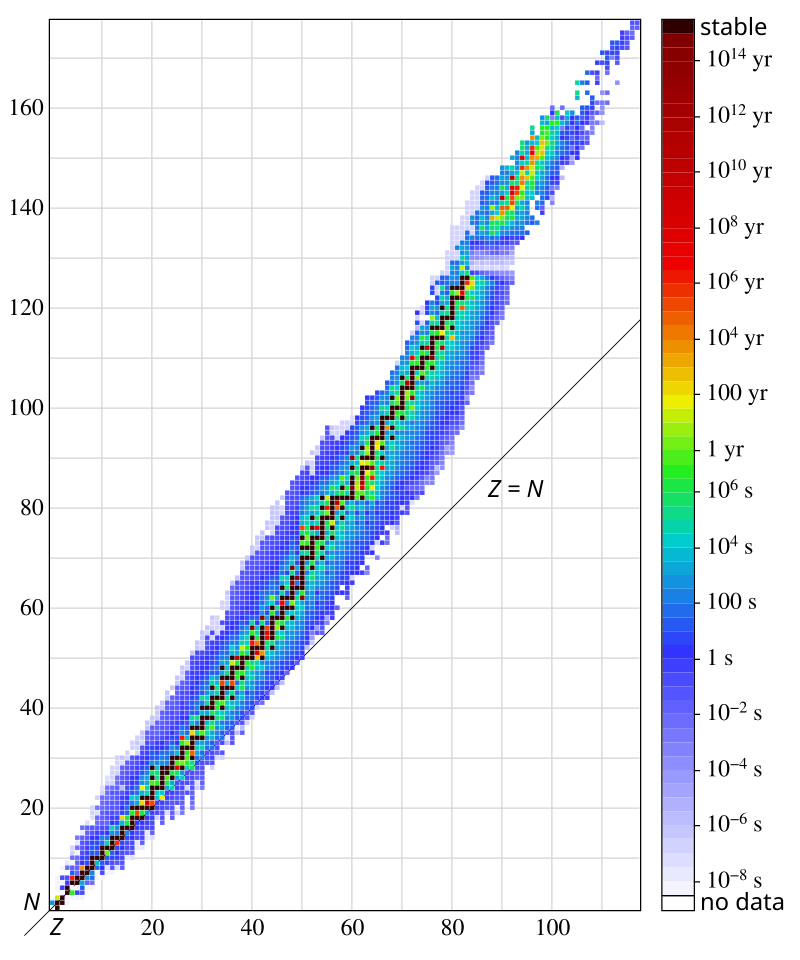
\includegraphics[width = 0.75\textwidth]{segre-chart.png}
  \caption{Tavola di Segré.}
  \label{segre-chart}
\end{figure}
\begin{figure}[h!]
  \centering
  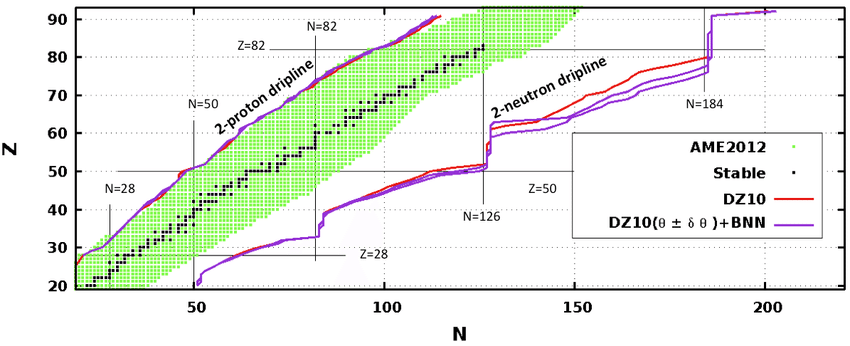
\includegraphics[width = 0.55\textwidth]{drip-lines.png}
  \caption{Nuclear driplines.}
  \label{drip-lines}
\end{figure}
\newpage











